\documentclass[12pt, a4paper]{article}

%%%%%%%%%%%%%%%紙張大小設定%%%%%%%%%%%%%%%
% \paperwidth=65cm
% \paperheight=160cm

%%%%%%%%%%%%%%%引入Package%%%%%%%%%%%%%%%
\usepackage[margin=1cm]{geometry} % 上下左右距離邊緣2cm
\usepackage{mathtools,amsthm,amssymb} % 引入 AMS 數學環境
\usepackage{yhmath}      % math symbol
\usepackage{graphicx}    % 圖形插入用
\usepackage{fontspec}    % 加這個就可以設定字體
\usepackage{type1cm}	 % 設定fontsize用
\usepackage{titlesec}   % 設定section等的字體
\usepackage{titling}    % 加強 title 功能
\usepackage{fancyhdr}   % 頁首頁尾
\usepackage{tabularx}   % 加強版 table
\usepackage[square, comma, numbers, super, sort&compress]{natbib}
% cite加強版
\usepackage[unicode, pdfborder={0 0 0}, bookmarksdepth=-1]{hyperref}
% ref加強版
\usepackage[usenames, dvipsnames]{color}  % 可以使用顏色
\usepackage[shortlabels, inline]{enumitem}  % 加強版enumerate
\usepackage{xpatch}

\graphicspath{ {images/} }
% \usepackage{tabto}      % tab
% \usepackage{soul}       % highlight
% \usepackage{ulem}       % 字加裝飾
\usepackage{wrapfig}     % 文繞圖
%\usepackage{lipsum}
% \usepackage{floatflt}    % 浮動 figure
\usepackage{float}       % 浮動環境
% \usepackage{caption}    % caption 增強
% \usepackage{subcaption}    % subfigures
% \usepackage{setspace}    % 控制空行
% \usepackage{mdframed}   % 可以加文字方框
% \usepackage{multicol}   % 多欄
% \usepackage[abbreviations]{siunitx} % SI unit
% \usepackage{dsfont}     % more mathbb

%%%%%%%%%%%%%%%%%%%TikZ%%%%%%%%%%%%%%%%%%%%%%
% \usepackage{tikz}
% \usepackage{circuitikz}

%%%%%%%%%%%%%%中文 Environment%%%%%%%%%%%%%%%
\usepackage[CheckSingle, CJKmath]{xeCJK}  % xelatex 中文
\usepackage{CJKulem}	% 中文字裝飾
\setCJKmainfont{Source Han Sans}
% 設定中文為系統上的字型,而英文不去更動,使用原TeX字型

% \XeTeXlinebreaklocale "zh"             %這兩行一定要加,中文才能自動換行
% \XeTeXlinebreakskip = 0pt plus 1pt     %這兩行一定要加,中文才能自動換行

%%%%%%%%%%%%%%%字體大小設定%%%%%%%%%%%%%%%
% \def\normalsize{\fontsize{10}{15}\selectfont}
% \def\large{\fontsize{40}{60}\selectfont}
% \def\Large{\fontsize{50}{75}\selectfont}
% \def\LARGE{\fontsize{90}{20}\selectfont}
% \def\huge{\fontsize{34}{51}\selectfont}
% \def\Huge{\fontsize{38}{57}\selectfont}

%%%%%%%%%%%%%%%Theme Input%%%%%%%%%%%%%%%%
% \input{themes/chapter/neat}
% \input{themes/env/problist}

%%%%%%%%%%%titlesec settings%%%%%%%%%%%%%%
% \titleformat{\chapter}{\bf\Huge}
            % {\arabic{section}}{0em}{}
% \titleformat{\section}{\centering\Large}
            % {\arabic{section}}{0em}{}
% \titleformat{\subsection}{\large}
            % {\arabic{subsection}}{0em}{}
% \titleformat{\subsubsection}{\bf\normalsize}
            % {\arabic{subsubsection}}{0em}{}
% \titleformat{command}[shape]{format}{label}
            % {編號與標題距離}{before}[after]

%%%%%%%%%%%%variable settings%%%%%%%%%%%%%%
% \numberwithin{equation}{section}
% \setcounter{secnumdepth}{4}  %章節標號深度
% \setcounter{tocdepth}{1}  %目錄深度
% \setcounter{section}{0}  %section 起始 counter
% \graphicspath{{images/}}  % 搜尋圖片目錄

%%%%%%%%%%%%%%%頁面設定%%%%%%%%%%%%%%%
\newcolumntype{C}[1]{>{\centering\arraybackslash}p{#1}}
\setlength{\headheight}{15pt}  %with titling
\setlength{\droptitle}{-2cm} %title 與上緣的間距
% \posttitle{\par\end{center}} % title 與內文的間距
\parindent=12pt %設定縮排的距離
% \parskip=1ex  %設定行距
% \pagestyle{empty}  % empty: 無頁碼
% \pagestyle{fancy}  % fancy: fancyhdr

% use with fancygdr
% \lhead{\leftmark}
% \chead{}
% \rhead{}
% \lfoot{}
% \cfoot{}
% \rfoot{\thepage}
% \renewcommand{\headrulewidth}{0.4pt}
% \renewcommand{\footrulewidth}{0.4pt}

% \fancypagestyle{firststyle}
% {
  % \fancyhf{}
  % \fancyfoot[C]{\footnotesize Page \thepage\ of \pageref{LastPage}}
  % \renewcommand{\headrule}{\rule{\textwidth}{\headrulewidth}}
% }

%%%%%%%%%%%%%%%重定義一些command%%%%%%%%%%%%%%%
\renewcommand{\contentsname}{目錄}  %設定目錄的標題名稱
\renewcommand{\refname}{參考資料}  %設定參考資料的標題名稱
\renewcommand{\abstractname}{\LARGE Abstract} %設定摘要的標題名稱

%%%%%%%%%%%%%%%特殊功能函數符號設定%%%%%%%%%%%%%%%
\DeclarePairedDelimiter{\abs}{\lvert}{\rvert}
\DeclarePairedDelimiter{\norm}{\lVert}{\rVert}
\DeclarePairedDelimiter{\inpd}{\langle}{\rangle} % inner product
\DeclarePairedDelimiter{\ceil}{\lceil}{\rceil}
\DeclarePairedDelimiter{\floor}{\lfloor}{\rfloor}
\DeclareMathOperator{\adj}{adj}
\DeclareMathOperator{\sech}{sech}
\DeclareMathOperator{\csch}{csch}
\DeclareMathOperator{\arcsec}{arcsec}
\DeclareMathOperator{\arccot}{arccot}
\DeclareMathOperator{\arccsc}{arccsc}
\DeclareMathOperator{\arccosh}{arccosh}
\DeclareMathOperator{\arcsinh}{arcsinh}
\DeclareMathOperator{\arctanh}{arctanh}
\DeclareMathOperator{\arcsech}{arcsech}
\DeclareMathOperator{\arccsch}{arccsch}
\DeclareMathOperator{\arccoth}{arccoth}
\newcommand{\np}[1]{\\[{#1}] \indent}
\newcommand{\transpose}[1]{{#1}^\mathrm{T}}
%%%% Geometry Symbol %%%%
\newcommand{\degree}{^\circ}
\newcommand{\Arc}[1]{\wideparen{{#1}}}
\newcommand{\Line}[1]{\overleftrightarrow{{#1}}}
\newcommand{\Ray}[1]{\overrightarrow{{#1}}}
\newcommand{\Segment}[1]{\overline{{#1}}}

%%%%%%%%%%%%%%%證明、結論、定義等等的環境%%%%%%%%%%%%%%%
\renewcommand{\proofname}{\bf 證明:} %修改Proof 標頭
\newtheoremstyle{mystyle}% 自定義Style
  {6pt}{15pt}%       上下間距
  {}%               內文字體
  {}%               縮排
  {\bf}%            標頭字體
  {.}%              標頭後標點
  {1em}%            內文與標頭距離
  {}%               Theorem head spec (can be left empty, meaning 'normal')

% 改用粗體,預設 remark style 是斜體
\theoremstyle{mystyle}	% 定理環境Style
\newtheorem{theorem}{定理}
\newtheorem{definition}{定義}
\newtheorem{formula}{公式}
\newtheorem{condition}{條件}
\newtheorem{supposition}{假設}
\newtheorem{conclusion}{結論}
\newtheorem{corollary}{推論}
\newtheorem{lemma}{引理}
\newtheorem{property}{性質}

\titlespacing*{\section} {0pt}{0ex}{0ex}

%%%%%%%%%%%%%%%Title%%%%%%%%%%%%%%%
\title{MLDS 2017 Spring HW1 - Language Model}
\author{B03901056 孫凡耕 B03901070 羅啓心\\
        B03901032 郭子生 B03901003 許晉嘉}
\date{\vspace{-5ex}}

\begin{document}
\maketitle 
\pagenumbering{gobble}% Remove page numbers (and reset to 1)
\thispagestyle{empty}
\section{Environment}
\begin{enumerate}
  \item 硬體資訊: 
    \begin{tabular}{|C{4cm}|C{3cm}|C{3cm}|C{3cm}|}
      \hline
      OS & CPU & GPU & Memory \\
      \hline
      \texttt{Arch linux 4.10} & \texttt{i7 3.4 GHz} &
      \texttt{GTX 1070}  & \texttt{32 GB}  \\
      \hline
    \end{tabular}
  \item 所使用的 \texttt{python} library:
    \begin{tabular}{|c|c|}
      \hline
      \texttt{spacy 1.6.0} & \texttt{nltk 3.2.2} \\
      \hline
    \end{tabular}
\end{enumerate}
% End of Environment

\section{Model description}
LSTM based RNN Language Model
\begin{enumerate}
  \item Performance:
    public score : \textbf{47.308 \%}, private score : \textbf{50.962\%}\\
  使用參數:\\
  \begin{tabular}{ll}
    word vector     & : glove.6B.300d \\
    rnn cell        & : full LSTM (with peephole) \\
    optimizer       & : Adam  \\
    clip gradient norm & : 5 \\
    sampled softmax & : used \\
  \end{tabular}
  \item 流程:\\
    \begin{tabular}{lcl}
      處理資料 & : & 將 Training data 轉成一個個單句或是以 dependency tree 的形式轉成若干單句,\\
               &   & 再將句子中每個單詞轉爲對應的 word vector。 \\
      訓練模型 & : & 使用變動長度多種的 rnn cell,輸入是除掉最後一個字的單句,輸出是通過  \\
               &   & softmax 之後與輸入算 loss,使用不同的 gradient descent 方法來訓練模型。\\
      測試資料 & : & 將 Testing data 以與 Training data 相同的方式進行處理,將各個選項填入的單 \\
               &   & 句個別丟入訓練完成的模型中,依據個別可能的機率來決定填空的答案。\\
    \end{tabular}
  \item 可調整之參數:\\
    \begin{tabular}{lcl}
      word vector & : & 使用的 word vector 來源及維度(選項:\texttt{glove.6B.50d}, \texttt{glove.6B.100d}, \\
                &  & \texttt{glove.6B.200d}, \texttt{glove.6B.300d}, \texttt{glove.42B.300d}, \texttt{glove.840B.300d})\\
      RNN layer & : & RNN 層數 \\
      softmax method: & : & softmax 方法(選項:\texttt{standard softmax}, \texttt{sampled softmax}, \texttt{nce loss}) \\
      sampled number & : & 在 sampled softmax 或 nce loss 中抽樣的 class 數目 \\
      optimizer & : & optimizers 的類型(選項:\texttt{GradientDescent}, \texttt{Adadelta}, \texttt{Adagrad},\\
                &   & \texttt{Momentum}, \texttt{Adam}, \texttt{RMSProp})\\
      rnn type & : & RNN Cell 的種類(選項:\texttt{Basic}, \texttt{basic LSTM}, \texttt{full LSTM}, \texttt{GRU}) \\
      learning rate & : & Learning rate 的大小 \\
      max grad norm & : & 所允許的 gradient norm 最大值,作爲 clipping 之用\\
      bidirectional & : & 是否使用 bidirectional RNN model\\
      epoch num & : & 一個 epoch 中總共使用多少個 batch\\
      train num & : & 總共使用 Holmes Training Data 中做 training 的檔案數目\\
      keep prob & : & Dropout layer 所使用的 keeping probability \\
      batch size & : &Training 時每個 batch 中 sentence 的數目\\
      hidden size & : & Hidden layer 的維度\\
    \end{tabular}
  \item 使用的外部資源:\\
     \begin{tabular}{lcll}
       Word vector & : & GloVe & (\href{https://nlp.stanford.edu/projects/glove/}{\url{https://nlp.stanford.edu/projects/glove/}}) \\
       Dependency Tree Parser & : & spacy & (\href{https://spacy.io/docs/usage/dependency-parse}{\url{https://spacy.io/docs/usage/dependency-parse}})
     \end{tabular}
\end{enumerate}
% End of Model description

\section{Improvement}
\begin{enumerate}
  \item 僅使用 Training Data 中,長度在特定範圍之內的句子\\
    特短的句子,大多屬於雜訊或是較無意義的短句(e.g. somebody said,);
    特長的句子,也均爲雜訊居多,若納入特長的句子亦會使 training model
    維度過高,造成記憶體空間不足。且特短及特長的句子,
    本身在 Training Data 中所佔的比例也不高(如 Figure ~\ref{fig:sentLenDis})。
    \begin{figure}[!htb]
      \centering
      \minipage{0.32\textwidth}
       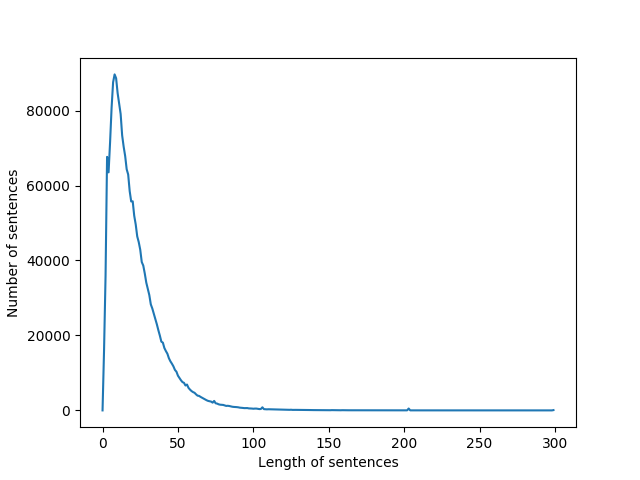
\includegraphics[scale=0.37]{sent_len_dis.png}
       \caption{句子長度分佈}
       \label{fig:sentLenDis}
      \endminipage\hfill
      \minipage{0.32\textwidth}
        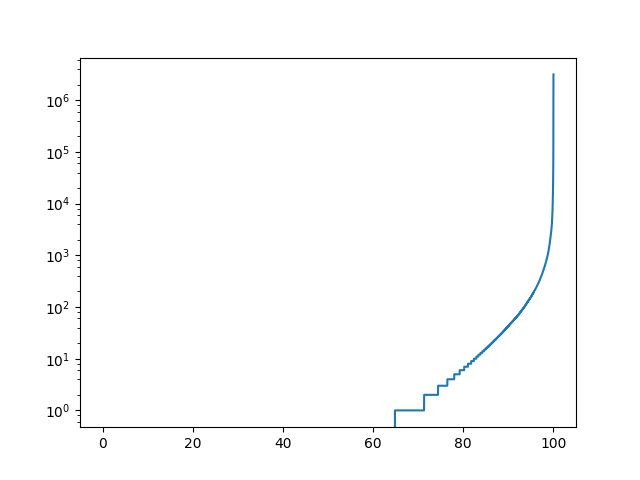
\includegraphics[scale=0.37]{word_dis2.png}
        \caption{單字出現次數分佈}
        \label{fig:wordDis2}
      \endminipage\hfill
      \minipage{0.32\textwidth}
        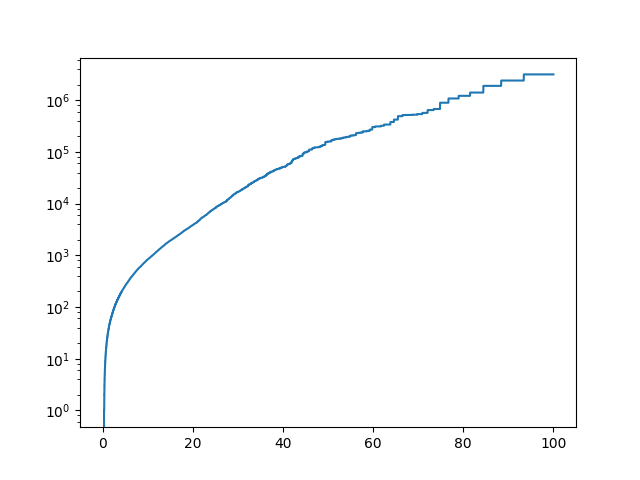
\includegraphics[scale=0.37]{word_dis.png}
        \caption{單字出現次數比例分佈}
        \label{fig:wordDis}
      \endminipage
    \end{figure}
  \item 將出現次數過少的單字從 corpus 中移除\\
    原本 corpus 的字量過大,會造成記憶體空間不足以及訓練困難,因此,將在
    Training Data 中出現次數較少的單字移除(視爲 unknown word),可使
    訓練學習的過程加速。從上圖 Figure ~\ref{fig:wordDis2} 
    可看出七成左右的單字不在 pretrained
    corpus 內或是出現次數少於兩次,而從 Figure ~\ref{fig:wordDis}
    可看出這些單字又僅佔不到
    總單字量的一個百分點,因此,將其刪除對於訓練的過程有較大的助益。
  \item 將 Training Data 中,開頭及結尾的部分刪去\\
    由於 Training Data 中幾乎所有文章,開頭及結尾皆相當於目錄或版權資訊等,
    較不爲一般常用語的句子。有利訓練過程的進行。
  \item Dependency Tree\\
    Dependency tree 可表示句子當中各單字之間的關聯。因此,將資料轉爲
    dependency tree 後,可更爲有效的分出每個句子中各個合法的語句,使訓練
    的資料更爲廣泛且一般。
    %舉例來說:對於句子\texttt{An inventory of syntactic functions is taken to be primitive.}
    %我們可以將其轉爲如圖 Figure ~\ref{fig:dt} 的 dependency tree。
    %\begin{figure}[!h]
      %\centering
      %\includegraphics[scale=0.5]{dt.png}
      %\caption{Dependency Tree}
      %\label{fig:dt}
    %\end{figure}
  \item Word Normalization\\
    在原先預處理 Training data 時,我們是利用 nltk 套件中的 sent tokenize
    以及 word tokenize,但由於 Training data 中,有些單字前後連接一些不重要
    的字元,形如:\texttt{'admit}、\texttt{.walk}、\texttt{*what}、等單字。
    而造成原本應是常用的單字,卻被我們判定成 unknown word 的情形。因此,我們
    將 nltk word tokenize 出來的單字,再進一步判斷,如果他包含兩個以上的英文
    字母,就將其他所有非英文字母的字元剔除。經過這一個正規化的步驟後,unknown
    word 的比例降低了 0.5\%,並且我們在 public score 上提升了 \textbf{7\%} !
  \item 加上 dropout 層 \\
    因為 3x512 的模型有點大,因此我們在 rnn 的 output layer 上加上 dropout 層,
    防止模型 overfitting,雖然 perplexity 降得稍微慢一點,但最終訓練出來的
    模型好壞較為穩定。
  \item 加上sampled softmax\\
    一開使用 standard softmax(呼叫 tensorflow 中的 sequence\_loss\_by\_example )
    訓練的速度較慢,通常需要訓練十幾個小時且結果也普通,換成 sampled softmax
    (呼叫 tensorflow 的 sampled\_softmax )之後訓練約 7 $\sim$ 8 個小時即可達到約 0.48 的結果。
\end{enumerate}
% End of Improvement

\section{Experiment}
除了嘗試不同的 model 以及各種 improvement,我們也針對以下幾種參數進行實驗,
除了試圖尋找最佳的參數,也嘗試驗證關於參數設定的各種傳聞。
\begin{enumerate}
  \item RNN Cell\\
    我們共嘗試了四種 RNN Cell,分別為 TensorFlow 1.0 所提供的:BasicRNNCell, 
    BasicLSTMCell, LSTMCell, 以及 GRUCell。其中 LSTMCell 不同於 basic 的版本
    是有使用 peep-hole。從 Figure ~\ref{fig:rnnType} 可以發現四種 cell 隨著 
    training epoch 數目的增加,perplexity 下降的幅度並無明顯差異,且基本上在
    經過一個 epoch 之後 perplexity 便無明顯變化,惟 BasicRNNCell 的振幅略大。
    儘管如此,在 private data score 的表現上,四種 cell 的分數依序是 
    0.40769, 0.46731, 0.48077, 0.46923,因此我們仍選擇有 peep-hole 的 
    LSTMCell 作為 model 中的 RNN cell。
  \item Learning Rate\\
    我們嘗試三種不同的 learning rate,分別為 0.1, 0.01, 0.001。由 Figure 
    ~\ref{fig:learningRate} 可以發現 learning rate 越大,perplexity 下降的速度也
    越快。然而正如同許多文獻所指出的:太大的 learning rate 可能無法到達 optimal 
    的點,這個說法亦在我們的實驗中得到驗證。
  \item RNN Layer 層數\\
    在 RNN model 中,我們除了使用單ㄧ層的 RNN cell,也有嘗試堆疊至 2 層及 3 層。
    由 Figure ~\ref{fig:layerTime} 可以發現 RNN cell 的層數越少, training 的速
    度越快,原因是參數較少的關係。三者在 private data score 上的表現別為
    0.47308, 0.48077,以及 0.49231,可以發現當 RNN cell 的層數為三層的時候,
    在這個 task 上有較佳的 performance。
  \item N-gram Model\\
    除了以上參數之外,我們也試圖做 model ensemble。其中包含 n-gram、pointwise
    mutual information (PMI) 等等。在 n-gram 的例子當中,$n = 1 \sim 4$ 於
    private data 的分數分別為 0.24615, 0.25962, 0.27885, 0.25769,其中 trigram 
    的表現最佳。由於我們發現在某些題目中,當空格代入不同的的選項時整句話所計算出
    的機率相同,因此我們認為或許是 Holmes training corpus 不夠大,使得許多 
    n-gram 的機率相同,因此沒有辦法有效提升分數。
  \item Pointwise Mutual Information (PMI)\\
    PMI 是我們嘗試使用的另一個 model,他的想法是將一個 sentence 先經過各種方法處
    理成為各種的 feature sets,這些 feature sets 包含的是一個 sentence 經過 
    filter 過後剩下的詞彙。得到 feature set 的方法有許多種,例如考慮 stop-word、
    使用 dependency tree、甚至只取空格前後兩個字等等。將處理完後的 feature sets 
    中的單字取出,根據 information theory 計算空格候選字與這些單字的關聯性,取出
    分數最高的即可。這個 model 在 MSR Sentence Completion Challenge 的分數表現高
    達 61.44\%,然而最終我們因為時間因素來不及完成。
    \begin{figure}[!htb]
      \centering
      \minipage{0.32\textwidth}
      \includegraphics[scale=0.37]{rnn_type_epoch.png}
      \caption{不同 RNN cell}
      \label{fig:rnnType}
     \endminipage\hfill
      \minipage{0.32\textwidth}
      \includegraphics[scale=0.37]{learning_rate_time.png}
      \caption{不同 learning rate}
      \label{fig:learningRate}
     \endminipage\hfill
      \minipage{0.32\textwidth}
      \includegraphics[scale=0.37]{layer_time.png}
      \caption{不同 RNN 層數}
      \label{fig:layerTime}
     \endminipage
    \end{figure}
\end{enumerate}
% End of Experiment

\section{Team division}
\begin{table}[h]
\centering
\begin{tabular}{ |C{2cm}|C{10cm}| }
  \hline
  孫凡耕 & 寫 RNN 模型、分配組內工作、教導組員\\
  \hline
  羅啓心 & 嘗試寫 Improvement、撰寫報告的模型描述\\
  \hline
  郭子生 & N-gram、跑實驗\\
  \hline
  許晉嘉 & 資料處理、PMI、統整撰寫報告、優化 kaggle 分數表現\\
  \hline
\end{tabular}
\end{table}
% End of Team division

\end{document}
